\section{Related Work}

\subsection{\cite{LabelingLanguageLearning}: In-Situ Labeling for Augmented Reality Language Learning}
%Huynh-2019 In-Situ Labeling for Augmented Reality Language Learning.
\cite{LabelingLanguageLearning} beschreiben ein Framework, mit dem die Lernmethode 'loci' in Augmented Reality umgesetzt werden kann. Die Lernmethode beruht darauf, Gegenstände der realen Welt mit Notizen zu beschriften. Für die Umsetzung mit AR wird eine automatische Echtzeit-Objekterkennung entwickelt. Dabei werden die Objekte auf RGB-Fotos der AR-Umgebung erkannt und in eine 3D-Rekonstruktion der Umgebung übernommen.

Die Lernmethode soll auf der AR-Brille 'Hololens' ausgeführt werden. Diese hat zu wenig Rechenleistung, um Object Detection durchzuführen. Daher wird eine Server-Client Architektur aufgesetzt. Die Kamera der AR-Brille nimmt ein Video der Umgebung auf. Die einzelnen Frames des Videos werden an den Server geschickt. Dieser nutzt ein neuronales Netzwerk, um alle erkennbaren Objekte in den Frames zu finden und mit Bounding-Boxen zu lokalisieren.

Für die Objekterkennung wird das neuronale Netzwerk von TensorFlow verwendet. Im Rahmen einer Analyse findet das Netzwerk mehrere Objekte in einem Foto. Die Objekterkennung soll in Echtzeit durchgeführt werden. Um die Laufzeit der Erkennung möglichst gering zu halten, wird die niedrigste Kameraauflösung mit 896x504 Pixel verwendet. Zusätzlich werden die Fotos als JPEG komprimiert. Auf diese Weise braucht die Analyse lediglich 30 ms pro Foto. So wird eine Echtzeit-Erkennung mit 30 Frames pro Sekunde möglich. Dennoch wird die Erkennung in der Applikation durch eine Netzwerk-Verzögerung von 150 ms zwischen der AR-Brille und dem Server verspätet.

Die AR-Brille 'Hololens' nummeriert die Frames, welche an den Server geschickt werden. Zusätzlich wird für jedes Frame die Kameraposition gespeichert, mit der es aufgenommen wurde. Aus diese Weise können Frames asynchron analysiert werden. Anschließend dienen die Bounding-Boxen der Objekte und die Kameraposition dazu, die Objekte in der 3D-Umgebung zu lokalisieren. Dafür wird der Mittelpunkt jeder Bounding-Box mithilfe eines Raycastes in die 3D-Szene projiziert.

Um Fehlern bei der Objekterkennung entgegenzuwirken, erfolgt die Markierung erst, wenn der Gegenstand auf mehreren Fotos gefunden wird. Durch die Analyse des ersten Fotos wird eine ungefähre Position in der AR-Umgebung für das Objekt ermittelt. Diese Position wird anschließend mit den Objekten verglichen, die während der nächsten 60 Frames erkannt werden. Falls Objekte gefunden werden, welche dieselbe semantische Bedeutung und eine ähnliche Position haben, wird davon ausgegangen, dass es sich um einen einzigen Gegenstand handelt, der in den 60 Frames mehrmals aufgenommen wurde. Siehe Abbildung \ref{img:60frames}.

\begin{figure}[H]
	\centering
	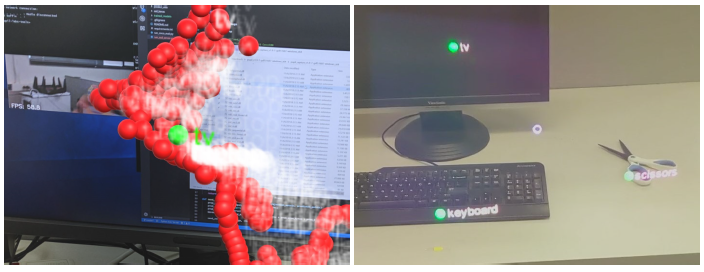
\includegraphics[width=0.8\textwidth]{images/img_huynh.PNG}
	\caption[Objekterkennung von \cite{LabelingLanguageLearning}]{Ungefähre Positionen des Objektes über 60 Frames aufgenommen in rot. Finale Position in grün.\citep{LabelingLanguageLearning}}
	\label{img:60frames}
\end{figure}

Unser Vorgehen zur Objekterkennung ähnelt dem Framework von \cite{LabelingLanguageLearning}. Auch hier soll die AR-Umgebung durch das Hinzufügen von Labels semantisch angereichert werden. Es wird ebenfalls ein neuronales Netz verwendet, um Object Detection auf RGB-Bildern durchzuführen. Wir haben dafür keinen eigenen Server aufgesetzt, sondern nutzen einen Cloud Service von Microsoft Azure. Durch Abspeichern von erhobenen semantischen Informationen ist eine Echtzeit-Detektion nicht relevant. Daher darf die Bild-Analyse länger dauern, was es erlaubt, mehrere neuronale Netze zu verwenden, die nach unterschiedlichen semantischen Informationen suchen.

In unserem Verfahren werden erkannte Objekte bereits in der Umgebung markiert, wenn sie nur ein einziges Mal erkannt wurden. Bei erneuter Aufnahme des Objektes, weist die zweite Analyse dem Objekt erneut die gleiche Klasse und eine ähnliche Position der AR-Umgebung zu. Daran lässt sich erkennen, das es sich um dasselbe Objekt handelt.

Die erste Position, die für das Objekt berechnet wurde, und die weitere Position, die aus der zweiten Aufnahme hervorgeht, unterscheiden sich mit hoher Wahrscheinlichkeit ein wenig voneinander. Daher wird der Mittelwert beide Positionen gebildet, um eine akkuratere Position für das Label des Objektes zu finden. Mit jedem neuem Bild wird so eine immer akkuratere  Position für das Label des Objektes ermittelt.
\citep{LabelingLanguageLearning}

%todo Die related work ist noch zu Kompakt - hier solltest du auch mehr über view management reden, und text labels - das paper von Bell ist schon was alt, da gibt es viel neues. Zb. mal schauen beim Joe Gabbard und Markus Tatzgern. Du solltest das kapitel vielleicht auch anfangen mit ein kurzen übersicht / zusammenfassung. 

\subsubsection{View Management}

In Augmented Reality Anwendungen werden häufig Objekte der realen Welt durch Labels mit Informationen annotiert. Die Labels können entweder 3D oder 2D-Elemente sein. Letztere befinden sich auf der Bildebene. Als Text-Label wird ein Schriftzug bezeichnet, der über eine Leader-Line mit einem Anchor verbunden ist. Der Anchor gibt die Position des Objektes in der Szene an, welches durch das Label beschriftet wird.

View Management ist das Erstellen eines Layouts für die Labels. Das Ziel besteht darin, die Labels gut lesbar auf der Bildebene zu positionieren und darzustellen. Dazu gehört, dass Labels sich gegenseitig nicht verdecken und auf eine verständliche Weise mit ihren Anchors verbunden sind. Einige View Management-Vorgehen legen auch Wert darauf, relevante Regionen der realen Welt zu bestimmen, die reich an Informationen oder für eine gegebene AR-Anwendung relevant sind. Diese Bereiche der realen Welt sollen nicht durch Labels verdeckt werden.

Es gibt viele Vorgehensweisen, um View Management umzusetzen. Sie unterscheiden sich je nachdem, ob sie ein Layout für 3D oder 2D-Labels erzeugen. Weiterhin unterscheiden sich die Vorgehensweisen darin, ob sie Wissen über die Geometrie der Szene nutzen (Geometry-Based) oder Fotos der Bildebene verwenden (Image-Based).

%greedy algorithmn oder force based algorithm werden eingesetzt, oder lerning based algorithms.

\citep{viewManagementGrasset} stellen ein Image-Based View Management-Vorgehen für 2D-Labels vor. Das Verfahren wird eingesetzt um Gebäude und Plätze der realen Welt mit 2D-Labels zu beschriften. Mit einer Aufnahme der Bildebene wird eine Saliency-Mag erzeugt. Diese gibt die Einzigartigkeit jedes Pixels an. Die Map wird mit einer Kantendetektion kombiniert, um eine Importance-Map zu erstellen. Letztere gibt an, wie informationsreich die Pixel sind. Mit der Importance-Map als Grundlage wird entscheiden, in welchen Bildbereichen Labels gesetzt werden können und welche Bildbereiche zu vermeiden sind.

Es wird eine Menge an Funktionen aufgestellt, mit denen die optimale Position eines Labels gefunden werden kann. Jede Funktion berechnet eine Wertung für ein gegebenes Label und eine Position der Bildebene im Hinblick auf die unterschiedlichen Ziele, welche ein Layout erfüllen soll. Dazu gehört, dass gewisse Bereiche der Importance-Map und der Kantendetektion-Map vermieden werden und dass Labels sich gegenseitig nicht verdecken sollen. Darüber hinaus soll die Distanz zwischen einem Label und seinem Anchor minimiert werden. Zudem kann eine favorisierte Richtung für die Leader Line angegeben werden, die den Look des Layouts beeinflusst. Mit einem Greedy Algorithmus wird die Position des Displays gefunden, an dem die Layout-Ziele, laut den Funktionen am besten erfüllt sind.
%springen von Labels?

%Um das Springen von Labels minimieren wird die berechnung des layouts mit einer nierigen frequenz ausgeführt. Die Labels werden nur an eine neue position gewegt, wenn sie besser ist als die alte und die labels werden mit einer smoothen animation zwischen positionen transitioned.

Zusätzlich zu dem Layout, welches die Positionen der Labels bestimmt, wird das Aussehen der Labels an ihren Hintergrund adaptiert, damit die Labels lesbar sind. Beispielweise erhalten die Leader-Lines eine unterschiedliche Farbe, abhängig von den Farben der Bildregionen, auf denen sie liegen.\cite{viewManagementGrasset} %Der Schriftzug eines Text-Labels hat ein background ein einen Background geben dessen lightness adaptiv ist. 


%für Augmented Reality Brower eine View Management Vorgehen entwickelt, das nicht darauf beruht, viel wissen über die Szene zu haben. 
%Vorgeben analysiert Video bilder um das Placement von Labels zu bestimmen und das Aussehen der Labels zu modifizieren.
%Labels so platziert, das wichtige infomration der realen Welt nicht versteckt wird, die Labels gut mit den objekten die sie annotieren sollen zusammenbleiben  und lesbarkeit der labels machen.
%
%
%
%
%
%
%andere works: geometry based layout oder image based layout
%
%geometrich based layout. haben wissen über den geometrischen aufbau der szene. ignorieren den view von realen objekten. beispiel davon ist Bell et al. 
%
%geometric based layout. layout of point features in goegraphic information systems and catography. NP hard problem. combined with image analysis. 
%
%image based layout
%learning based approcha um gute regionen zu finden in denen in AR ein Label platziert werden kann. Importance Maps aus video bildern. kann auch contraints an die positoinen der labels geben und dynamische labels machen.
%


%<old>
%
%\cite{viewmanagement3d} beschreiben View Management für interaktive 3D Benutzeroberflächen. Als View Management wird die Positionierung von Labels bezeichnet.
%Die Labels können sich auf eine 2D Ebene beschränken oder im 3D Raum liegen. View Management zielt darauf ab die Labels so zu positionieren, dass sie einander und relevante reale Objekte nicht verdecken. Gleichzeitig sollen die Labels die Gegenstände der realen Welt auf eine verständliche Art annotieren. Labels sollen nahe bei den Objekten liegen, zu denen sie gehören. Siehe Abbildung \ref{viewManagement}.
%
%\begin{figure}[H]
%	\centering
%	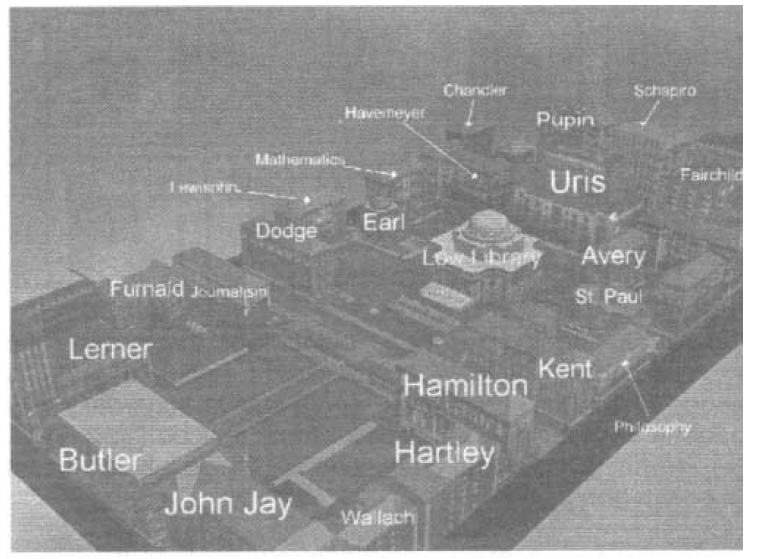
\includegraphics[width=0.7\textwidth]{images/img_viewmanagement.PNG}
%	\caption[View Management von \cite{viewmanagement3d}]{3D Labels durch View Management positioniert.\citep{viewmanagement3d}}
%	\label{viewManagement}
%\end{figure}



Unsere Applikation würde durch View Management profitieren. Nach der Erkennung eines Gegenstandes in der Umgebung erfolgt eine Markierung in dem 3D-Raum durch ein 3D-Label. Die Lesbarkeit der Labels kann durch View Management verbessert werden, indem ihre Positionen über die Zeit verändert werden. 

Das Layout der Labels müsste auf Veränderungen des Betrachtungswinkels und auf Hinzukommen von neuen Labels reagieren. Idealerweise würden keine Informationen verdeckt werden. Labels sollten weder andere Labels noch Gegenstände der realen Welt verdecken. Besonders sollte darauf geachtet werden, dass Objekte, welche durch ein Label annotiert werden, nicht verdeckt sind.

View Management geht jedoch über den Rahmen dieser Arbeit hinaus und kann daher nicht umgesetzt werden. %\citep{viewmanagement3d,viewmanagement}



\subsection{\cite{contextawaremixedreality}: Context-Aware Mixed Reality: A Framework for Ubiquitous Interaction}

\cite{contextawaremixedreality} stellen ein Framework vor, das einer AR-Umgebung semantische Eigenschaften zuweist, um realistische Interaktionen zwischen virtuellen und realen Objekten zu erreichen. 
Insbesondere sollen physikalische Interaktionen an Realismus gewinnen.

Das Framework reichert die Umgebung mit Informationen über die Materialien an, aus denen reale Oberflächen und Gegenstände in der Umgebung bestehen. Die Umgebung wird in einer 3D-Szene durch ein Mesh repräsentiert. Die einzelnen Voxel des Meshes werden mit Labels annotiert, um ihnen Semantik zuzuweisen.

Als beispielhafte Applikation wird ein First-Person-Shooter vorgestellt, bei dem das Aussehen von Einschusslöchern davon abhängt, auf welches Material geschossen wird. Siehe Abbildung \ref{img:game}.

\begin{figure}[h]
	\centering
	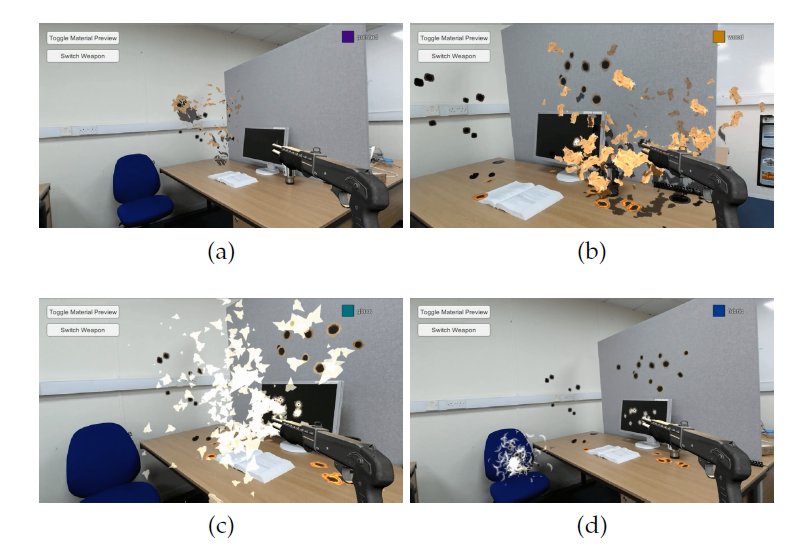
\includegraphics[width=0.8\textwidth]{images/img_shootinggame.png}
	\caption[Context Aware Shooter von \cite{contextawaremixedreality}]{Es gibt unterschiedliche Interaktionen, wenn auf eine Wand (a), einen Tisch (b), einen Bildschirm (c) und einen Stuhl (d) geschossen wird.\citep{contextawaremixedreality}}
	\label{img:game}
\end{figure}

Für die Erkennung der Materialien werden mehrere Frames der AR-Brille 'Hololens' segmentiert. Die dadurch entstehenden semantischen Informationen werden abgespeichert, um bei späteren Interaktionen der AR-Applikation abrufbar zu sein. Die Erkennung der Materialien ist nicht echtzeitfähig. Die Interaktionen können dennoch in Echtzeit ablaufen, da sie auf bereits gespeicherte Materialien-Informationen zugreifen. 

RGB-Bilder der Umgebung werden aufgenommen und mit einem neuronalen Netzwerk analysiert, um semantische Informationen zu erheben. Das neuronale Netz wird von \cite{contextawaremixedreality} für den First-Person-Shooter aufgesetzt. Das Netz wurde darauf trainiert, 23 unterschiedliche Materialien - beispielsweise Holz, Glas, Stoff etc. - zu erkennen und Bilder nach ihnen zu segmentieren. Dabei wird für jedes Pixel ein Material angegeben.

Mithilfe der Kamera-Position des Frames werden die Material-Informationen auf ein 3D-Modell der Umgebung, ähnlich einer Textur, projiziert. Als Resultat wird an jedes Voxel des 3D-Modells ein Label pro Frame gehängt, das die semantischen Informationen wiedergibt, die in dem Frame erkannt wurde.

Bei der Segmentierung können Fehler auftreten, indem das auf dem Foto erkannte Material nicht dem realen Material entspricht. Um diesen Fehlern entgegenzuwirken werden mehrere Frames aufgenommen und analysiert. %Bildbereich, die schwer einzuordnen sind, werden in unterschiedlichen Frames unterschiedlich segmentiert. 

Die Informationen aus den Frames bilden sich auf die Voxel ab. Durch die Kumulierung der Segmentierungen erhält jedes Voxel eine Menge an Labels. Voxel, die in schwer einzuordnenden Bildbereichen liegen, erhalten Labels, die unterschiedliche Informationen beinhalten. Um sicherzustellen, dass jedes Voxel des 3D-Modells nur eine semantische Bedeutung hat, werden die gesetzten Labels mit einer Baysian-Fusion und einem neuronalen Netz überarbeitet. Als Resultat hat jedes Voxel nur ein einziges Label.

Unser Verfahren versucht ebenfalls, das Verständnis der AR-Umgebung durch semantische Informationen zu erweitern. Auch wir nutzen ein neuronales Netzwerk, um RGB-Fotos der Umgebung zu analysieren.
In unserem Verfahren erhält nicht jedes Pixel semantische Informationen, sondern nur solche Pixel, welche die Position eines Gegenstandes markieren. Daher haben nur ausgewählte Voxel des 3D-Meshes ein Label.\citep{contextawaremixedreality}

\newpage
\section{Grundlagen}
\subsection{Grundlagen zu Augmented Reality}
\subsubsection{Augmented Reality}

Augmented Reality vermischt die reale Welt mit digitalen (virtuellen) Elementen, um dem Nutzer eine erweiterte Wahrnehmung zu ermöglichen. Es können 3D-Objekte, 2D-Overlays oder Audioelemente verwendet werden, um eine reale Umgebung mit Informationen zu bereichern. 

Die Umgebung beinhaltet den Teil der realen Welt, welcher in Augmented Reality abgebildet und erweitert werden soll. Umgebung kann beispielsweise ein Zimmer sein, in dem eine AR-Anwendung ausgeführt wird. Die AR-Umgebung umfasst sowohl die reale Umgebung als auch die virtuellen Elemente.

Augmented Reality weist drei grundlegende Merkmale auf, die ein möglichst nahtloses Verschmelzen der realen Welt mit den virtuellen Elementen unterstützen: 
\begin{itemize}
	\item Die Realität wird mit dem Virtuellen kombiniert. Dazu werden reale Elemente mit Virtuellen überlagert.
	\item Interaktion mit virtuellen Elementen erfolgen in Echtzeit.
	\item Virtuelle Elemente haben einen festen räumlichen Platz in der AR-Umgebung.
\end{itemize}

In einer AR-Umgebung kann navigiert werden, indem der Nutzer sich physikalisch durch die reale Umgebung bewegt. Die reale Welt und die virtuellen Elemente stehen dabei immer in demselben räumlichen Verhältnis zueinander. Für AR ist die einzige Möglichkeit der Navigation. Andernfalls würde die Verschmelzung der virtuellen Elemente mit der realen Welt schlechter gelingen.

Da die reale Welt immer zu sehen ist, gibt sie sowohl eine Referenz als auch einen Kontext für die virtuellen Objekte an. 
Beispielsweise steht die Größe von virtuellen Objekten immer in Relation zu der realen Umgebung.\citep{GrundlagenAR}

\subsubsection{AR-System}

Ein AR-System besteht aus der Hard- und Software, die benötigt wird, um eine AR-Umgebung zu erzeugen. Es muss die Vermischung der realen Welt mit virtuellen Elementen anzeigen. Darüber hinaus muss es sowohl die Interaktionen des Nutzers mit virtuellen Elementen als auch die Interaktionen von virtuellen Elementen mit der realen Welt simulieren.

Ein AR-System ist in der Regel nicht an einen bestimmten Ort gebunden, sondern kann in unterschiedlichen Umgebungen eingesetzt werden, die diverse reale Gegenstände aufweisen. AR-Applikationen müssen in der Lage sein, die unterschiedlichen Umgebungen zu unterstützen.\citep{GrundlagenAR}

%book Virutal reality chapter 1

\subsubsection{Grundlagen zu 3D-Szenen für AR}

Die digitalen Inhalte der AR-Anwendung werden in einer virtuellen Szene gespeichert. 
AR-Anwendungen müssen in Echtzeit laufen. Daher muss die virtuelle Szene echtzeitfähig sein. Im besten Fall kann ein Nutzer keine Zeitverzögerung  zwischen der virtuellen Welt und der realen Welt bemerken.

Um Interaktionen mit digitalen Elementen zu ermöglichen, werden relevante Teile der realen Welt in der 3D-Szene repräsentiert. 
So werden beispielsweise die Wände und der Boden eines Raumes in der Szene abgebildet. Auch die Position eines Controllers und die Blickrichtung des Nutzers kann mithilfe von Sensoren verfolgt und in die Szene einbezogen werden.

\subsubsection{Spatial Mapping} 
Um virtuelle Objekte an eine Umgebung anzupassen und Interaktion zwischen virtuellen Objekten und der realen Welt zu ermöglichen, benötigt ein AR-System Informationen über die Geometrie der Umgebung. Mit den Sensoren der AR-Hardware werden Informationen gesammelt, welche Aussagen über die Geometrie der Umgebung treffen. Beispielsweise haben AR-Geräte eine Tiefenkamera, welche Entfernungen messen kann. Die Daten der Sensoren werden gesammelt und in Relation zu der Bewegung des Gerätes gesetzt, um die Umgebung zu rekonstruieren. Dieser Vorgang nennt sich 'Spatial Mapping'. 

Mit Hilfe der entstehenden 'Spatial Map' können digitale Elemente mit der Umgebung interagieren. Zudem wird die 'Spaital Map' bei der Darstellung der digitalen Elemente verwendet, um zu entscheiden, wie digitale Elemente die Umgebung verdecken oder von ihr verdeckt werden.\citep{spatialMapping} 

\begin{figure}[H]
	\centering
	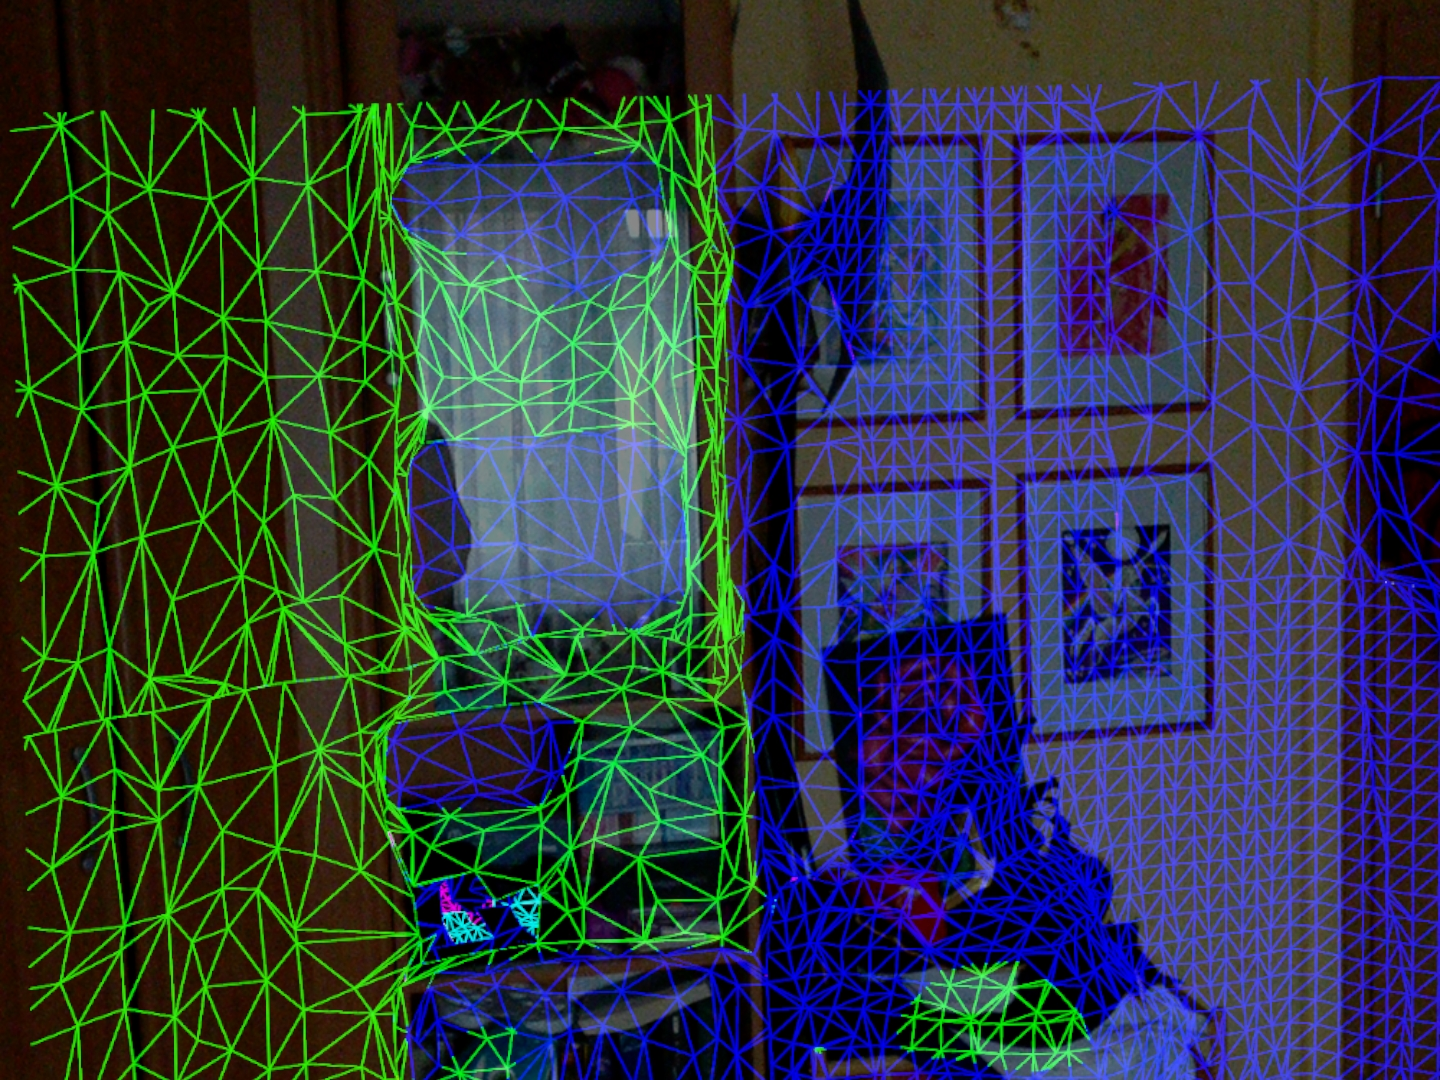
\includegraphics[width=0.7\textwidth]{images/ML_20201003_15.36.42.jpg}
	\caption[Spatial Mapping]{Spatial Map. Die Farben des Meshes zeigen die Entfernung des Nutzers zu den Objekten an.}
	\label{img:spatialmap}
\end{figure}

\subsection{Magic Leap AR-Brille}

Die 'Magic Leap One Lightwear' ist eine Augmented Reality-Brille, die von dem Unternehmen 'Magic Leap' entwickelt wurde. Sie verfügt über ein Head-Mounted Display und eine Recheneinheit, welche über ein Kabel mit dem Display verbunden ist. Die transportable Recheneinheit kann an der Hüfte getragen werden, was die AR-Brille mobil macht. 


\subsubsection{Hardware}

Die Recheneinheit besitzt zwei 'Denver 2.0 64 Bit' Prozessor-Kerne und vier 'ARM Contex A57 46 bit' Kerne. Davon sind einer der 'Denver' Kerne und zwei der 'ARM Contex' Kerne für Applikationen nutzbar.  

Die AR-Brille besitzt neun Sensoren und mehrere Kameras. Dazu gehören:
\begin{itemize}
	\item ein Infrarot Tiefen-Sensor,
	\item ein Eye Tracker,
	\item eine Foto- und Videokamera, die im Format 16:9 mit einer Auflösung von 1920x1080 Pixeln aufnimmt und
	\item mehrere Umgebungskameras die in unterschiedliche Richtungen ausgerichtet sind. \citep{mlofficialsalespitch,mlglossary}
\end{itemize}

Der Output geschieht über ein Display mit einem 50 Grad Field of View und einem Seitenverhältnis von 4:3. Das Display ist transparent. Daher kann die reale Welt immer betrachtet werden. Selbst wenn ein weißes Objekt angezeigt wird, schimmert die reale Welt noch durch. 

Eingaben erfolgen über einen 6 Degree of Freedom Controller. Er verfügt über 3 Knöpfe (Trigger, Bumper, Home Button) und ein Touchpad. \citep{mlofficialsalespitch,mlglossary}

\begin{figure}[H]
	\centering
	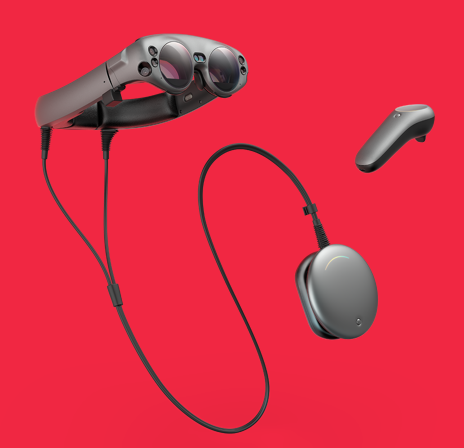
\includegraphics[width=0.7\textwidth]{images/img_magicLeap.PNG}
	\caption[Magic Leap One AR-Brille.\citep{mlImage}]{Magic Leap One AR-Brille.\citep{mlImage}}
	\label{magcileap}
\end{figure}

\subsubsection{Betriebssystem}
Die 'Magic Leap' Brille läuft auf dem Betriebssystem 'Lumin OS'. Dieses wurde für Augmented Reality entwickelt und bietet Applikationen entsprechende Funktionalitäten an. Beispielsweise führt das Betriebssystem Spatial Mapping durch.\citep{mlluminOS,mlluminfeatures}

Dabei werden mit den Sensoren und Kameras der Brille Daten aufgenommen und in einen zeitlichen Zusammenhang mit der Bewegung der Brille gesetzt, um eine Rekonstruktion des Raumes zu erhalten.\citep{mlluminOS,mlluminfeatures,mlluminworldreconstruktion,mlmeshingunity}

Lumin OS bietet es Applikationen an,
\begin{itemize}
	\item Raycasts auf die Umgebung durchzuführen und
	\item ein Mesh der Rekonstruktion zu erhalten.
\end{itemize}
Neben dem Spatial Mapping unterstützt Lumin OS die Verarbeitung des Contorller-Inputs und die Verwaltung der Zugriffsrechte von Applikationen. Dazu gehört beispielsweise das Recht (die Permission), die Fotokamera und das Netzwerk zu nutzen.\citep{mlluminfeatures,mlappsecurity}

Selbst wenn mehrere Applikationen das Recht zur Kameranutzung haben, kann zu jedem Zeitpunkt nur eine Applikation auf die Fotokamera zugreifen. Die Applikationen müssen sich mit der Kamera-Ressource von Lumin OS verbinden. Diese reguliert, welche der Applikationen eine Fotoanfrage stellen darf und das aufgenommene Foto erhält. 


\subsubsection{Unity Applikationen für Magic Leap One}
Unity ist eine Entwicklungsumgebung, mit der Applikationen für Lumin OS erstellt werden können. Ein Unity Projekt besteht aus mindestens einer Szene, in der mehrere 'GameObjects' existieren. 'GameObject' ist ein Oberbegriff für alle Elemente, die in der Szene existieren. Sie bilden eine hierarchische Struktur, in der GameObjects Parents oder Children weiterer GameObjects sind.\citep{unitygameobject}

GameObjects haben weder eine Funktionalität noch ein Aussehen. Beides wird durch Components hinzugefügt. Einige Components sind bereits in Unity integriert. So erhält jedes GameObject eine Transform Component, die ihm eine Position in der Szene gibt. Darüber hinaus können Components mithilfe eines Mesh Renderers einem GameObject eine sichtbare 3D-Form geben. Components können auch komplexere Verhalten implementierten. Beispielsweise kann ein GameObject als Kamera der Szene fungieren. Um eine neue Funktionalität hinzuzufügen, kann ein C\# Script geschrieben und einem GameObject als Component zugewiesen werden.

Magic Leap unterstützt die Entwicklung von Applikationen für Lumin OS mit Unity. So wird ein Unity Project Template von Magic Leap angeboten, welches das Set-up der Applikation erleichtert. Dazu gehören die Build-Optionen des Projektes und die Einstellung der Hauptkamera 'Unity Kamera'. Letztere rendert die Szene für das Display der AR-Brille 'Magic Leap One'. Die Kamera verfolgt die Bewegungen der Magic Leap Brille und kopiert diese in der Unity Szene. \citep{mlgetstarted}%Die Szene bleibt somit stationär und die Kamera bewegt sich in ihr, so wie der Nutzer der Magic Leap sich in einer Umgebung bewegt.

Das Unity Template verfügt über vorgefertigte Skripts, die auf Funktionalitäten von Lumin OS zugreifen:

\begin{itemize}
	\item \textit{MLInput} stellt Informationen über den Controller zur Verfügung. Damit können die Knöpfe und Touchpad-Gesten überwacht werden.\citep{mlinput}
	\item \textit{MLCamera} greift auf die Fotokamera der AR-Brille zu. Fotoanfragen und Resultat-Daten werden ebenfalls durch MLCamera behandelt.
	\item \textit{MLPrivilegeRequestBehavior} ermöglicht es den Nutzer nach dem Recht zu fragen, auf bestimmte Teile des AR-Systems zuzugreifen. Beispielsweise muss nach Permission gefragt werden, um die Fotokamera-Ressource zu verwenden.\citep{mlprivileges}
	\item \textit{MLRaycast} greift auf die Spatial Mapping Funktionalitäten von Lumin OS zu. Somit kann ein Raycast auf die Rekonstruktion der Umgebung beim Betriebssystem in Auftrag gegeben werden. Ein Raycast ist ein Strahl, welcher sich durch einen 3D-Raum bewegt. Der Ursprung und die Richtung des Strahles müssen angegeben werden. Objekte, die einen Schnittpunkt mit dem Strahl aufweisen, gelten als 'vom Raycast getroffen'.\citep{unityraycast,mlraycast}
	\item \textit{MLSpatialMapper} zeigt die Rekonstruktion der Umgebung von Lumin OS als Mesh an. Dieses besteht aus GameObjects, welche von \textit{MLSpatialMapper} erzeugt werden. Das Mesh wird ständig aktualisiert, um das geometrische Verständnis des Betriebssystems widerzuspiegeln.\citep{mlluminworldreconstruktion,mlmeshingunity}
\end{itemize}

Scripts können von der Klasse \textit{Monobehavior} erben. \textit{Monobehaviors} verfügen über Methoden, die von Unity zu unterschiedlichen Events der Laufzeit ausgeführt werden. Nur Skripts, die ein Component eines GameObjects sind, werden aufgerufen. Folgende Methoden können unterschieden werden:

\begin{itemize}
	\item \textit{Awake} wird aufgerufen, wenn das GameObject initialisiert wird. %Wenn ein GameObject initialisiert wird, werden die Awake() Methoden der Componenten aufgerufen.
	\item \textit{Update} wird zu jedem Frame der Anwendung aufgerufen.
	\item \textit{OnDestroy} wird aufgerufen, wenn das GameObject aus der Szene gelöscht wird.
\end{itemize}

\textit{Monobehaviors} können über globale Variablen verfügen. Wenn das Skript einem GameObject als Component angehört, kann der Inhalt der globalen Variable in Unity modifiziert werden. Dies eröffnet die Möglichkeit, einem Skript eine Referenz auf ein bestimmtes GameObject zu geben. Siehe Abbildung \ref{img:gloabvars}.

\begin{figure}[H]
	\centering
	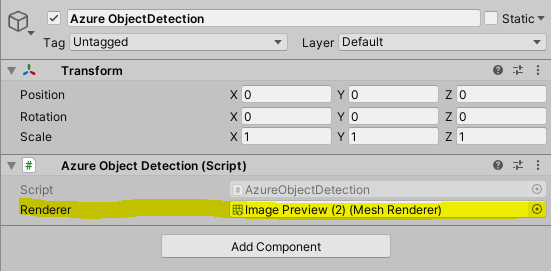
\includegraphics[width=0.8\textwidth]{images/img_globalVars.png}
	\caption[Unity GameObject mit Components]{GameObject mit Components. Das Component 'Azure Object Detection' verfügt über eine globale Variable, welche auf eine Mesh Renderer Component eines anderen Objektes verweist.}
	\label{img:gloabvars}
\end{figure}


\textit{Monobehaviors} können als Singleton fungieren, indem sie eine globale statische Referenz auf sich selbst anlegen, wenn ihre \textit{Awake} Methode aufgerufen wird.%Siehe Abbildung \ref{code:singleton}.

\begin{lstlisting}
public class MySingletonClass : MonoBehavior
{
	public static MySingletonClass instance = null;
	private void Awake()
	{
		if (instance != null && instance != this)
		{
			Destory(this.gameObject);
		}
		instance = this;
	}
	public void DoSomething(){...}
}
\end{lstlisting}

%\begin{figure}[H]
%	\centering
%	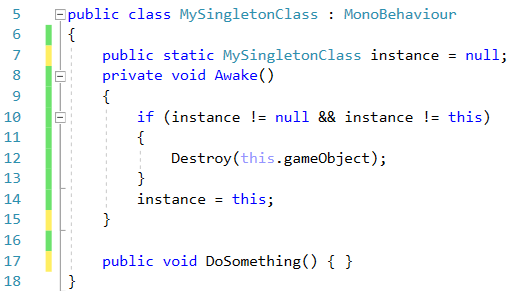
\includegraphics[width=0.7\textwidth]{images/code_singleton.png}
%	\caption[Quellcode Singleton Klasse]{Quellcode einer Singleton Klasse}
%	\label{code:singleton}
%\end{figure}

Jedes andere Script kann die Instanz des Singletons aufrufen, indem es die statische Referenz der Klasse des Singletons verwendet. %Siehe Abbildung \ref{code:singleton2}.
\begin{lstlisting}
MySingletonClass.instance.DoSomething();
\end{lstlisting}
%\begin{figure}[H]
%	\centering
%	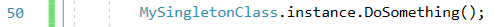
\includegraphics[width=0.7\textwidth]{images/code_singleton2.png}
%	\caption[Quellcode Aufrug des Singletons]{Quellcode Aufruf des Singletons}
%	\label{code:singleton2}
%\end{figure}

Skripts können während der Laufzeit GameObjects erzeugen. Um festzulegen, wie das GameObject aussehen soll, kann in dem Unity Editor ein 'Prefab' erstellt werden. 'Prefabs' sind vorgefertigte, abgespeicherte GameObjects, deren Child Objects, Components und globale Variablen festgelegt werden. Das Prefab fungiert als Vorlage für GameObjects, die zur Laufzeit initialisiert werden. Während der Initialisierung wird eine Position der Szene angegeben, an welche das neue GameObject angefügt wird. Nachdem das Objekt initialisiert wurde, kann auf seine Components und Scripts zugegriffen werden.\citep{unityprefabs}


\subsubsection{Lokale und globale Koordinatensysteme in 3D-Szenen}
%\newline
In der 3D-Szene werden die Positionen von Objekten als Matrizen in dreidimensionalen Koordinatensystemen verwaltet. Es gibt ein globales Koordinatensystem (auch 'Weltkoordinatensystem' oder 'World Space' genannt), in welchem alle Objekte relativ zu einem Ursprung liegen. 

Jedes Objekt hat zusätzlich ein eigenes, lokales Koordinatensystem (Objektkoordinatensystem). Dessen Ursprung liegt in dem jeweiligen Objekt. Die Position und Rotation des Objektes in dem globalen Koordinatensystem bestimmt die Relation zwischen dem globalen und dem lokalen Koordinatensystem. 

Das lokale Koordinatensystem einer Kamera wird auch 'Camera Space' genannt. Die Relation zwischen dem Camera Space und dem globalen Koordinatensystem wird in Unity durch die \textit{cameraToWorld} Matrix beschrieben. Mithilfe dieser Matrix kann eine Koordinate aus dem Camera Space in die entsprechende Koordinate des globalen Koordinatensystems transformiert werden. Dazu wird die Koordinate als Vektor angegeben und mit der cameraToWorld Matrix multipliziert. Das Resultat ist ein Vektor, welcher eine Koordinate im globalen Koordinatensystem angibt.\citep{unitycameratoworldmatrix,unitymultiplyoint}

\subsubsection{Kamera in 3D-Computergrafik}
\paragraph{View Frustum}
ist das Teilvolumen einer 3D-Szene, welche auf einen zweidimensionalen Bildschirm abgebildet wird. Alle Objekte, die von der Kamera gesehen werden, befinden sich in dem View Frustum.

\paragraph{Clipping Plane}
bezeichnet eine Ebene, welche den View Frustum quer zur Blickrichtung begrenzt. Es gibt eine vordere und eine hintere Clipping Plane. Die vordere Clipping Plane liegt nah an der Kamera. Alle Objekte, die zwischen der Kamera und der vorderen Clipping Plane liegen, werden nicht angezeigt. Die hintere Clipping Plane limitiert, wie weit Objekte entfernt sein können, bevor sie nicht mehr zu sehen sind. Siehe Abbildung \ref{dia:clipping}.\citep{unityclipping}

\begin{figure}[H]
	\centering
	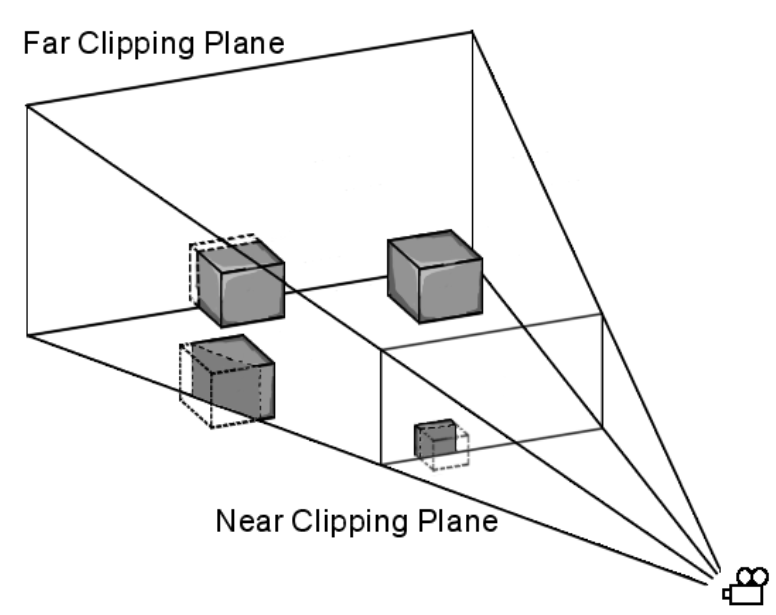
\includegraphics[width=0.7\textwidth]{images/dia_ViewFrustum.png}
	\caption[View Frustum]{Diagramm des View Frustum mit Clipping Planes.}
	\label{dia:clipping}
\end{figure}

%to myself: yay :) you're doing well I believe in you!

\subsection{Computer Vision}
Computer Vision hat zum Ziel, die Inhalte digitaler Bilder und Videos zu verstehen. Sowohl semantische als auch geometrische Inhalte werden dabei analysiert. 
Zu den Aufgaben von Computer Vision gehören Objekterkennung und Bildsegmentierung.

In diesem Bereich kommen Statistik, Bilderverarbeitung und maschinelles Lernen zum Einsatz. Maschinelles Lernen wird eingesetzt, um neuronale Netze zu formen, welche in der Lage sind Bild- und Videoanalysen durchzuführen
.\citep{intortodeeplearingmedical}

\subsubsection{Object Detection}

Objekt Detection ist eine Aufgabe der Computer Vision. Es sollen mehrere Objekte in einem Bild erkannt werden. Daher wird auch der Name 'Image Based Object Detection' verwendet. Spezialisierungen von Object Detection sind beispielsweise Gesichtserkennung oder das Erkennen von Fußgängern. Durch eine Objekterkennung werden semantische Inhalte eines Bildes automatisch erhoben. 

Für die Objekte werden sowohl eine Klasse als auch eine Bounding-Box bestimmt. Die Klasse gibt an, um welche Art von Objekt es sich handelt. So wird Beispielsweise angegeben, ob es sich um eine Tastatur oder einen Computerbildschirm handelt (Object Classification). Die Bounding-Box gibt ein Viereck in dem Bild an, in welchem sich das Objekt befindet(Object Localization). \citep{objectdetection,objectDetectionReview}



%todo Eventuell kannst du auch noch kurz was zur objekterkennung dort einpacken (das sind allerdings schon sehr alte paper ;) Das letzte geht aber auch im 3.3.1
\subsubsection{Artificial Neural Networks}
'Artificial Neural Networks' sind Machine-Learning-Architekturen, welche beispielsweise Musik, Text oder Bilder nach Mustern durchsuchen. Artificial Neural Networks sind für keine genaue Aufgabe programmiert, sondern lernen indem sie mit Beispieldaten trainiert werden. Jedem Beispiel wird ein Label zugeordnet, welches angibt, ob das gesucht Muster in dem Beispiel vorhanden ist. Die Struktur des Networks verfügt über Gewichte, welche Einfluss auf den Output haben. Mit jedem Trainingsbeispiel passt das Network die Gewichte an, sodass der Output dem Label des Beispiels entspricht.\citep{introToCNN,surveyOfDeepLearing}

Artificial Neural Networks bestehen aus einer Menge an miteinander verbundenen Knoten, die jeweils eine Berechnung durchführen. Diese Knoten sind in Ebenen aufgeteilt. Unterschieden wird: ein Input Layer, mehrere Hidden Layer und ein Output Layer. Die Knoten einer Ebene sind mit allen Knoten der vorherigen Ebene verbunden.\citep{introToCNN,surveyOfDeepLearing}

Das Neural Network bekommt eine Menge an Daten als Input. Die Knoten arbeiten zusammen, um den Output zu erzeugen. Jeder einzelne Konten führt eine Berechnung durch. Mithilfe von Gewichten wird entschieden, wie viel Einfluss das Rechenergebnis der einzelnen Knoten auf die nächste Ebene hat.\citep{introToCNN,surveyOfDeepLearing}

Um ein Neural Network zu trainieren, wird der Output von einem Mensch bewertet. Das Neural Network nutzt diese Bewertung, um die Gewichte der einzelnen Knoten zu verändern. So passt sich das Neural Network an. \citep{introToCNN,surveyOfDeepLearing}

\subsubsection{Convolutional Neural Networks}
'Convolutional Neural Networks' sind auf das Verarbeiten von Bildern spezialisiert. Sie nutzen aus, dass Bilder viele Redundanzen und informationsarme Bereiche haben. Daher können mit jedem Verarbeitungsschritt des Networks Informationen weggelassen werden, um Rechenzeit und Volumen der Trainingsdaten zu verringern.\citep{introToCNN,surveyOfDeepLearing,cNNforClass}

Convolutional Neural Networks sind Machine-Learning-Architekturen, die darauf ausgelegt sind, Muster in Bildern zu erkennen. Sie müssen auf das zu erkennende Muster trainiert werden. Dazu wird ihnen eine Menge an Beispielbildern gegeben, die teilweise das Muster erhalten. Für jedes Beispiel wird der gewünschte Output angegeben, der erreicht werden soll. Die Struktur des Network verfügt über Gewichte, welche die Berechnung des Outputs beeinflussen. Mit jedem Trainigsbild passt das Network die Gewichte an, damit die Muster korrekt erkannt werden.\citep{introToCNN,surveyOfDeepLearing}

Die Knoten in einer Ebene eines Convolutional Neural Networks sind nur mit wenigen Knoten der vorherigen Ebene verbunden. So sinkt die Menge an Informationen mit jeder Ebene. Das CNN wird gezwungen, sich auf wesentliche Teile des Bildes zu konzentrieren, mit denen beispielsweise ein Objekt oder  Muster erkannt werden kann. \citep{introToCNN,surveyOfDeepLearing}

\subsubsection{Azure Computer Vision Services}

'Microsoft Azure' ist eine Cloud-Computing-Plattform, welche im Jahr 2010 von Microsoft eingeführt wurde. Ihr Ziel ist es, Cloud-Services zur Verfügung zu stellen, die unter anderem Computer Vision Aufgaben durchführen. Diese sind über 'REST-APIs' erreichbar. 

Eine 'REST-API' ist eine Programmierschnittstelle, die sich an dem Verhalten des World Wide Webs orientiert. 'REST' steht für 'Representation State Transfer' und bezeichnet einen Architekturansatz für die Kommunikation zwischen verteilten Systemen. REST verlangt unter anderem ein Client-Server-Modell und eine zustandslose Kommunikationen zwischen Client und Server. Jede Anfrage eines Clients beinhaltet alle Informationen, welche für die Antwort des Servers relevant sind.

Eine Rest-API kann mit http/s realisiert werden. Eine HTTP-Anfrage (HTTP-Request) wird verwendet, um auf eine Funktion eines Servers zuzugreifen. Dabei wird der Server durch seine Web URL angesprochen. Diese wird auch 'Endpoint' genannt. HTTP-Methoden, wie 'GET' und 'POST' teilen dem Service mit, welche Funktion durchgeführt werden soll. Mit der Methode 'GET' werden Daten von dem Server angefordert. Die Methode 'POST' erlaubt die Übermittlung von zusätzlichen Daten an der Server.

Ein HTTP-Request besteht aus: einer 'Start Line', einer Menge an 'Headers' und einem 'Body'. Die 'Start Line' gibt die HTTP-Methode und die Endpoint-URL an.
In den 'Headers' werden weitere Informationen über die Anfrage an den Server angegeben. Für die Anwendung einer API, wird der Authentifizierungsschlüssel des Clients in einem 'Header' gespeichert.
Zuletzt hat der Request einen 'Body'. Abhängig von der HTTP-Methode ist der 'Body' entweder leer, oder er beinhaltet Daten für den Server. So speichert eine POST-Nachricht ihre Daten, beispielsweise ein Foto in dem 'Body'. Die Länge und Art der Daten wird mit 'Headern' angegeben.
  
Jeder HTTP-Anfrage wird eine 'HTTP-Response' als Antwort zurückgeschickt. 
Die 'HTTP-Response' besteht ebenfalls aus einer 'Start Line', 'Headern' und einem 'Body'. Die 'Start Line' gibt einen Responce-Code und einen Statustext an. Der Responce-Code teilt dem Client mit, ob die Anfrage erfolgreich bearbeitet wurde. Wenn ein Error aufgetreten ist, gibt der Responce-Code Auskunft über die Art des Errors. Der Statustext gibt eine kurze Erklärung des Responce-Codes.

Beispiel Response-Codes:
\begin{itemize}
	\item 404 - Url nicht gefunden
	\item 401 - Zugriff verweigert wegen ungültiger Authentifizierung
	\item 400 - fehlerhafte Anfrage. Der Service konnte die Anfrage nicht verstehen
	\item 200 - Anfrage wurde erfolgreich bearbeitet
\end{itemize}

Bei erfolgreicher Bearbeitung beinhaltet der Body die Antwort auf die HTTP-Anfrage.

\subsubsection{Azure Object Detection}
Microsoft Azure bietet einen Computer Vision Service an. Dabei handelt es sich um mehrere Künstliche-Intelligenz-Modelle, die für unterschiedliche Aufgaben trainiert wurden. Dazu gehört unter anderem ein Service für Object Detection. Dabei sendet der Anwender ein Bild an Microsoft. Der Service verarbeitet das Bild und schickt dem Anwender ein Ergebnis in Form einer Json-Datei zurück.\citep{getAzure,whatIsAzure,objDetectAzure,Azure302Doc}

Die Object Detection basiert auf einem trainierten KI-Modell. Dieses weist unter anderem folgende Limitierungen auf: Zum einen kann es nur Objekte erkennen, für die es trainiert wurde. Zudem können Objekte nicht erkannt werden, die in dem Foto sehr klein sind oder nah bei anderen Objekten liegen.\citep{azureobjdetec}

Der Object Detection Service ist durch eine REST-API erreichbar. Durch eine POST-Anforderung wird eine Analyse angefragt. In dem Body der HTTP-Anfrage werden dabei die Bilddaten übertragen. Die Response-Nachricht beinhaltet eine Json-Datei, welche die gefundenen Objekte und deren Positionen auf dem Foto beinhaltet. Um den Object Detection Service zu nutzen, wird eine HTTP Post-Anforderung an die Webadresse geschickt. Als Endpoint wird die Webadresse der REST-API angegeben. Die Nachricht muss folgenden Inhalt haben:
\begin{itemize}
	\item Ein Authentifizierungsschlüssel, der mit einem Azure Account verbunden ist
	\item und Bilddaten
\end{itemize}

Das Resultat der Bildanalyse wird in der Response-Nachricht zurückgeschickt. Der Response-Code 200 gibt an, dass die Analyse erfolgreich durchgeführt wurde. In diesem Falle wird eine Json-Datei mitgeschickt. Beispiel:

\begin{lstlisting}
{"objects":[{"rectangle":{"x":1377,"y":900,"w":157,"h":138},"object":"computer mouse","confidence":0.681},
{"rectangle":{"x":1336,"y":0,"w":584,"h":841},"object":"display","confidence":0.873},
{"rectangle":{"x":315,"y":25,"w":906,"h":622},"object":"display","confidence":0.839},
{"rectangle":{"x":447,"y":800,"w":862,"h":166},"object":"computer keyboard","confidence":0.71}],
"requestId":"a77e261a-7d40-4159-bf78-19d8fb61ad92",
"metadata":{"height":1080,"width":1920,"format":"Jpeg"}}
\end{lstlisting}

Die gefundenen Objekte befinden sich in der Liste mit dem Key 'objects'. Jedes Element der Liste hat ein Bounding-Box 'rectangle' und eine Klassenbezeichnung 'object'. Zusätzlich hat jedes Objekt einen 'confidence' Score. Dieser gibt die Wahrscheinlichkeit an, dass das Objekt korrekt erkannt wurde. 
Zusätzlich zu den Objekten werden eine requestId und Metadaten über das Bild zurückgeschickt.

\subsubsection{Azure Custom Vision}
Mit 'Azure Custom Vision' bietet Microsoft auch ein untrainiertes Object Detection KI-Modell an. Dieses muss vor dem Einsatz von einem Nutzer trainiert werden. Custom Vision kann als Ergänzung zu Azure Object Detection verwendet werden, da es für spezifische Objekte trainiert werden kann. \citep{Azure302bDoc}

Über eine Webseite lässt sich der Trainingsprozess des Modells steuern und auswerten. Der Nutzer lädt Fotos hoch und fügt jedem Foto händisch einen oder mehrere Tags hinzu. Jeder Tag repräsentiert eine Art von Gegenstand (Objekt-Klasse). Um einem Foto ein Tag anzufügen, muss eine rechteckige Region des Fotos markiert werden, in welchem der jeweilige Gegenstand zu sehen ist. Siehe Abbildung \ref{img:trainingone}.

\begin{figure}[H]
	\centering
	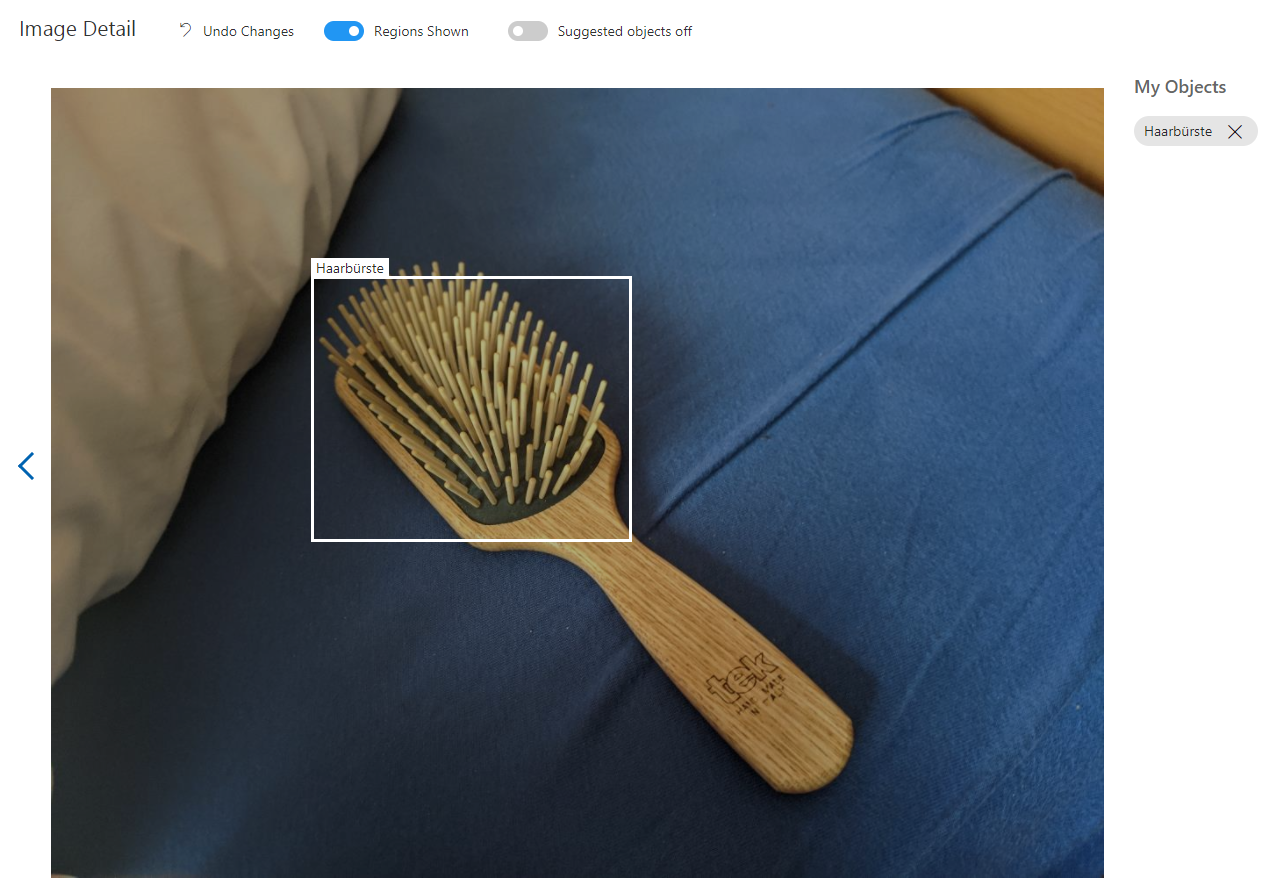
\includegraphics[width=1\textwidth]{images/trainingone.png}
	\caption[Trainingsbild für Azrue Custom Detection]{Trainingsbild für die Objekterkennung einer Haarbürste.}
	\label{img:trainingone}
\end{figure}

Für jede Objekt-Klasse müssen mindestens 15 Bilder hochgeladen werden, in welchen der entsprechende Tag vorkommt. Anschließend kann der Trainingsprozess gestartet werden. Eine größere Anzahl von Bildern in dem Trainingsset erhöht die Genauigkeit der Objekterkennung. Azure empfiehlt die Verwendung von mindestens 50 Bildern pro Tag. Bei einer geringen Anzahl von Trainingsbildern haben die einzelnen Bilder einen sehr großen Einfluss auf das Modell.

Durch das Training wird eine 'Iteration' des Modells erzeugt. Diese kann verwendet werden, um Object Detection durchzuführen. Bei jedem Start eines neuen Trainingsprozesses, wird eine weitere Iteration erstellt. Alle Iterationen werden unter einer eindeutigen Projekt-ID gespeichert und während einer Testphase evaluiert. Für jede Objekt-Klasse in einer Iteration werden die folgenden drei Metriken angesetzt:
\begin{itemize}
	\item Precision - bezeichnet die Wahrscheinlichkeit, dass ein gefundenes Objekt, tatsächlich der angegeben Klasse angehört. (Die Wahrscheinlichkeit, dass es kein false positive ist.)
	\item Recall - greift aus einer Menge an Objekten, die einer Klasse angehören, den Prozentsatz an Objekten heraus, der von dem Modell korrekt lokalisiert und klassifiziert wurde.
	\item A.P (Average Precision) - bezeichnet eine Gesamtwertung für die Evaluierung basierend auf Precision und Recall. 
\end{itemize}

Die Evaluierungen der einzelnen Objekt-Klassen werden in Precision, Recall und Mean Average Percision gemittelt. Siehe Abbildung  \ref{img:trainineval}.

\begin{figure}[H]
	\centering
	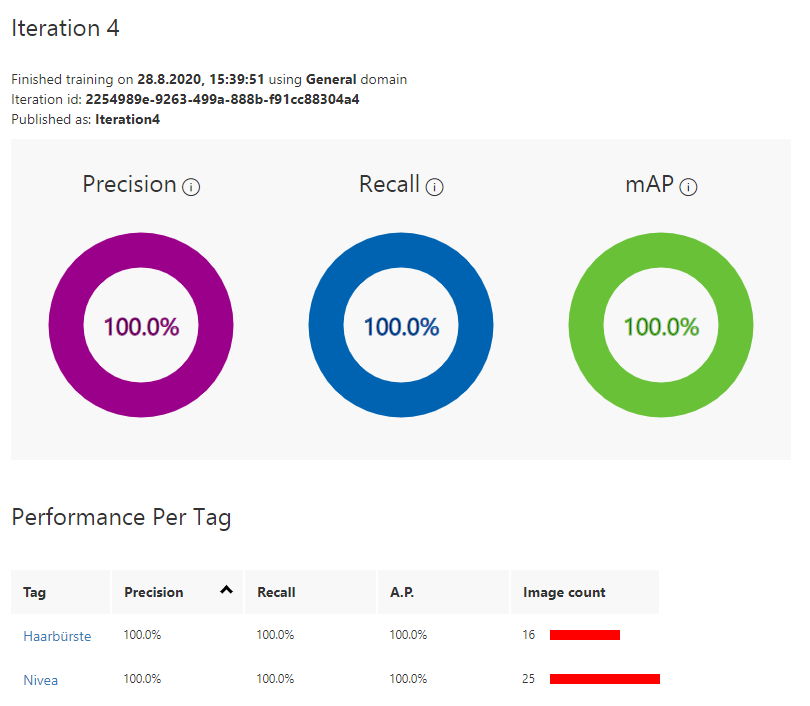
\includegraphics[width=1\textwidth]{images/trainingevaluation.png}
	\caption[Evaluierung eines Azure Custom Detection Modells]{Die Evaluierung des Modells}
	\label{img:trainineval}
\end{figure}

Mit einer erzeugten Iteration des Modells kann eine Object Detection durchgeführt werden. Der Custom Vision Service ist durch eine REST-API erreichbar. Der Endpoint beinhaltet die ID des Projektes und die Nummer der Iteration, welche verwendet werden soll. In der POST-Nachricht werden sowohl ein Authentifizierungsschlüssel als auch ein Bild mitgeschickt, welches von der Iteration analysiert werden soll.

Das Resultat der Analyse ist eine Json-Datei. 
Der Aufbau der Datei unterscheidet sich ein wenig von dem Dateiaufbau der Azure Object Detection.  

\begin{lstlisting}
{"id":"9cb0cc50-1dca-4b4a-b4d1-95d6bd25c352",
"project":"ac915246-5268-461f-bd11-cf0c1826d509",
"iteration":"2254989e-9263-499a-888b-f91cc88304a4",
"created":"2020-10-10T02:40:40.107Z",
"predictions":[{"probability":0.997380137,"tagId":"d390d34e-afc4-4ff4-8dcd-3ee8fe79cb8f","tagName":"Haarbürste","boundingBox":{"left":0.258805573,"top":0.226171583,"width":0.303168833,"height":0.329167157}},
{"probability":0.0141124222,"tagId":"d390d34e-afc4-4ff4-8dcd-3ee8fe79cb8f","tagName":"Haarbürste","boundingBox":{"left":0.542580664,"top":0.507969,"width":0.2195471,"height":0.3491398}},
{"probability":0.0116642443,"tagId":"263b3042-8958-4775-9a19-e2602d19c9b7","tagName":"Nivea","boundingBox":{"left":0.542580664,"top":0.507969,"width":0.2195471,"height":0.3491398}}]}
\end{lstlisting}

In der Antwort werden Informationen über die Iteration wiedergegeben, welche für die Analyse genutzt wurde. Die gefundenen Objekte werden in der Liste "predictions" aufgezählt. Die Objektklasse wird in "tagName" gespeichert. Die "probability" gibt das Vertrauen des Modells darin an, dass das Objekt korrekt erkannt wurde. Die erkannten Objekte müssen nach ihrer Probability gefiltert werden, da auch Objekte mit einer sehr niedrigen Probability in der Json Datei enthalten sind. 